\documentclass[a4paper,openright,12pt]{book}
%\documentclass[b5paper,openright,11pt]{book}
\usepackage[utf8]{inputenc}
\usepackage{graphicx,color}
\usepackage[dvipsnames]{xcolor}
\usepackage{amsfonts}
\usepackage{amsmath}
\usepackage{amssymb}
\usepackage{verbatim}
\usepackage{cite} 
\usepackage{fancyhdr}
\usepackage{epigraph}
\usepackage{caption}
\usepackage{psfrag}
\usepackage{hyperref}
\usepackage{pdfpages}
\usepackage{setspace}
\usepackage{tikz}
\captionsetup[figure]{font=footnotesize,labelfont=footnotesize}
\graphicspath{{../figures/}}
%To use a kind of times new roman font style
\usepackage{mathptmx}
\usepackage{newtxtext,newtxmath}
\usepackage[titletoc]{appendix}
%To modify the space before title of each chapter
%\usepackage{titlesec}
%\titleformat{\chapter}[display]   
%{\normalfont\huge\bf}{\chaptertitlename\ \thechapter}{20pt}{\Huge}   
%\titlespacing*{\chapter}{0pt}{-10pt}{40pt}
%Modificar encabezado y pie de página.
\pagestyle{fancy}
\fancypagestyle{chapters}{%
\fancyhead{}
\fancyhead[LE,RO]{\thepage}
\fancyhead[RE]{Nanoscale hydrodynamics near solids}
\fancyhead[LO]{{\color{Gray}CHAPTER \thechapter } \leftmark }
\fancyfoot{}
\renewcommand{\headrulewidth}{0.5pt}
}
%\fancyfoot[LE,RO]{\thepage}
%\fancyfoot[LO,CE]{Chapter \thechapter}
%\fancyfoot[CO,RE]{Author Name}
\fancypagestyle{noHeader}{%
\fancyhead{}
\renewcommand{\headrulewidth}{0pt}
}

%New commands
\renewcommand\bibname{References}
\renewcommand{\thefootnote}{\roman{footnote}}
\newcommand{\esc}{\!\cdot\!}
\newcommand{\Note}[1]{{\bf \color{red}#1}}    % comments and notes
\newcommand{\Pep}[1]{{\color{blue}#1}}     % del libro de Pep
\newcommand{\Pendiente}[1]{{\color{green}#1}} % Revisar
\newcommand{\Tirar}[1]{{\color{Magenta}#1}}   % tirar
\newcommand{\llangle}{\left\langle}
\newcommand{\rrangle}{\right\rangle}
\newcommand{\llg}{\left\lgroup}
\newcommand{\rlg}{\right\rgroup}
\newcommand{\bra}{\llbracket}
\newcommand{\ket}{\rrbracket}
\newcommand{\cc}{\!\parallel\!}
\newcommand{\GK}[2]{\langle#1 \cc #2\rangle}
\newcommand{\GKrest}[2]{\langle#1 \cc #2\rangle^0}


% Second and third pages

\newcommand{\firstpage}{
  \thispagestyle{empty}

      \begin{flushright}
        
\includegraphics[height=64pt]{logoED}
      \end{flushright}
      \vspace*{\fill}
      
      \vspace{5pt}
      \begin{center}
        \textsc{\Huge{Tesis Doctoral}}\\
      
      \vspace{20pt}
      
      \textsc{\Huge{2019}} \\
      \vspace{40pt}
      
      
      %\noindent{\rule{\textwidth}{1pt}}\par
      \textsc{\Huge{Nanoscale hydrodynamics \\near solids}}
      \noindent{\rule{\textwidth}{1pt}}\par
      
      \vspace{20pt}
      \textsc{\Large{Diego Duque Zumajo}} \\
      
      %\vspace{20pt}
      %\textsc{\large{Master Universitario en Energías y Combustibles del futuro}} \\
      
      \vspace{50pt}
      %\tikz[remember picture,overlay] \node[opacity=0.1,inner sep=0pt] at (current page.center){\includegraphics[width=0.6\paperwidth,height=0.6\paperwidth]{escudoUNED}};
      \tikz[remember picture,overlay] \node[opacity=0.1,inner sep=0pt] at (0,3) {
\includegraphics[width=0.6\paperwidth,height=0.6\paperwidth]{EscudoUNED}};
      
      \vspace{15pt}
      \textsc{\Large{Programa de doctorado en Ciencias}} \\
      \vspace{20pt}
      \textsc{\large{Director: Dr. Pep Español Garrigós}} \\
      \end{center}
      
      
      \vspace*{\fill}
      }
      \renewcommand{\maketitle}{
      \firstpage
}

\newcommand{\copyrightpage}{
        \newpage
        \thispagestyle{empty}
        \begin{flushright}
        
\includegraphics[height=48pt]{logoED}
        \end{flushright}
        \vspace*{\fill}
        
        {\scshape \noindent Doctoral dissertation at the Department of
        Fundamental Physics in the Faculty of Science, UNED.}
        \vspace{0.5em}
        
        \noindent \begin{tabular}{lp{10cm}}
        \noindent {\bf  Title:}  & Nanoscale hydrodynamics near solids\\
        \noindent {\bf Author:} & Diego Duque Zumajo
        , M. Sc. in Energies and Fuels for the future. \\
        \noindent {\bf Director:} & Dr. Pep Español Garrigós.
        \\
        \end{tabular}
        \vspace*{\fill}
        
        {\scshape \noindent Tesis doctoral presentada en el Departamento
        de Física Fundamental de la Universidad Nacional de Educación a Distancia.}
        \vspace{0.5em}
        
        \noindent \begin{tabular}{lp{10cm}}
        
        \noindent {\bf Título:} &  Hidrodinámica cerca de paredes. \\
        \noindent {\bf Autor:} & Diego Duque Zumajo, Máster Universitario en Energías y Combustibles para el futuro. \\
        \noindent {\bf Director:} & Dr. Pep Español Garrigós.\\
        \end{tabular}
        \vspace*{\fill}
        
        
        %\noindent\rule{\textwidth}{0.1em}
        %\begin{center}
        %  
\includegraphics[scale=0.1]{by-nc-sa} \\
        %\scshape \noindent \small \copyright \ \small Diego Duque Zumajo, 
        %2019 \\
        %This work is licensed under a Creative Commons
        %Attribution-NonCommercial-ShareAlike 4.0 International \\
        %(CC BY-NC-SA 4.0) License.
        %\end{center}
        %\newpage
        %\rm
        }

\begin{document}
\maketitle
\copyrightpage
\spacing{1.5}
\newpage
\pagenumbering{Roman} % para comenzar la numeracion de paginas en numeros romanos


\chapter*{Acknowledgments} % si no queremos que añada la palabra "Capitulo"
\pagestyle{noHeader}  %define page style for the chapters
%\addcontentsline{toc}{chapter}{Agradecimientos} % si queremos que aparezca en el índice
%\markboth{Acknowledgments}{Acknowledgments} % encabezado 

\tableofcontents % indice de contenidos

\chapter*{Abstract} % si no queremos que añada la palabra "Capitulo"
\pagestyle{noHeader}  %define page style for the chapters
%\addcontentsline{toc}{section}{Abstract} % si queremos que aparezca en el índice
%\markboth{Abstract}{Abstract} % encabezado


\chapter*{Resumen} % si no queremos que añada la palabra "Capitulo"
%\pagestyle{noHeader}  %define page style for the chapters
%\markboth{Resumen}{Resumen} % encabezado
Esta tesis doctoral estudia el comportamiento nanoscópico de un fluido  cuando entra en contacto con un sólido. Derivaremos las ecuaciones de movimiento de un fluido en contacto con una esfera sólida de grandes dimensiones. Emplearemos la técnica de los operadores de proyección de Kawasaki-Gunton y asumiremos un comportamiento Markoviano. Abordaremos el problema del plateau presente en la expresiones de Green-Kubo que aparecen en las ecuaciones de la hidrodinámica, ofreciendo una expresión corregida para la expresión de Green-Kubo sin el conocido problema del plateau. 


Posteriormente discretizaremos las ecauciones obtenidas para poder hacer mediciones mediante simulaciones de dinámica molecular y abordaremos el caso más sencillo posible, es decir, un fluido en condiciones de contorno periódicas. 


Emplearemos la teoría de Mori para obtener una expresión que nos de la evolución temporal de las correlaciones del momento tranversal del fluido. 
Comportamiento Markoviano si esas correlaciones decaen de forma exponencial. 

Estudiaremos el comportamiento Markoviano de un fluido confinado. Tamaño de los bines. 


Finalmente obtendremos la condición de contorno del fluido y el sólido. 


\chapter*{Copyright holder, notation and quotes}
\pagestyle{noHeader}  %define page style for the chapters

This dissertation is presented as a compendium of publications. The articles included in each chapter correspond to the postprint version of the publications (i.e. the final version without the publisher layout) as follows:  

\begin{itemize}
  \item Chapter 1 corresponds to the postprint version of the article \textit{Nanoscale hydrodynamics near solids} published in \textit{The Journal of Chemical Physics}. DOI 10.1063/1.5010401
  \item Chapter 2 corresponds to the postprint version of the article \textit{A solution to the plateau problem in the Green-Kubo formula} published in \textit{Physical Review E}. DOI 
  \item Chapter 3 corresponds to the postprint version of the article \textit{Discrete hydrodynamics I: Theory for planar flows with confinig walls} published in \textit{}. DOI
  \item Chapter 4 corresponds to the postprint version of the article \textit{Discrete hydrodynamics II: Space and time locality for unconfined fluids} published in \textit{}. DOI 
  \item Chapter 5 corresponds to the postprint version of the article \textit{Discrete hydrodynamics III: Non-Markovian behaviour near solid walls} published in \textit{}. DOI 
  \item Chapter 6 corresponds to the postprint version of the article \textit{Discrete hydrodynamics IV: The slip bpundary condition} published in \textit{}. DOI 
  \end{itemize}

Although the notation we use is indicated in the articles, we remark that functions of microstates z in phase space are denoted with a hat as in $\hat{A}(z)$. We follow this convention except for probability densities, as in $\rho_t(z)$. Operators are denoted with ${\cal CALIGRAPHIC}$ symbols. Vectors and matrices are denoted with {\bf boldfaces}.
%We use a number of superscripts for matrices. $M^T$ is the transpose of $M$ , $M^S = (M+M^T )/2$ is the symmetric part of the matrix M while $M^A = (M-M^T )/2$ is the antisymmetric part. 

%Sometimes we follow Einstein summation convention in which, for example the product of two matrices in components is written as
%\begin{align}
%    (AB)_{\mu\nu} = A_{\mu\nu}B_{\nu\sigma}=\sum_{\nu}A_{\mu\nu}B_{\nu\sigma} \nonumber
%\end{align}
%The derivative of a composite function is expressed as
%\begin{align}
%    \frac{\partial}{\partial x}F(g(x))=\frac{\partial F}{\partial g}(g(x))\frac{\partial g}{\partial x}(x) \nonumber
%\end{align}

The quotes in the beginning of each chapter are taken from books I read over the time I have spent working in this dissertation, the last four years. I have respected the language in which the writter wrote the book. 


%\tableofcontents % indice de contenidos

%\pagenumbering{arabic}
%\setcounter{chapter}{-1}

%--------------------
%- INTRODUCTION
%--------------------

%\setcounter{chapter}{-1}
\singlespacing
\chapter{Introduction}\label{Chap:Intro}
\pagenumbering{arabic}
\pagestyle{noHeader}  %define page style for the chapters
\markboth{Introduction}{Introduction}
\epigraph{\textit{There is no future. There is no past. Do you see? Time is simultaneous, an intricately structured jewel that humans insist on viewing one edge at a time, when the whole design is visible in every facet.}}{Watchmen \\ ALAN MOORE} 
%No hay futuro. No hay pasado ¿Lo ves? El tiempo es simultáneo, una joya de una estructura demasiado compleja en donde los humanos se empeñan en solo ver un borde, cuando el diseño por completo es visible en todas las facetas.-Alan Moore.
\spacing{1.5}
It was in the nineteen century when the Statistical Mechanics (SM) was born mainly because of the work of Ludwing Boltzmann and Josiah Willard Gibbs. The goal was to reconcile the Thermodynamics with the microscopic laws. 

Thermodynamics was well-established because it draws its concepts from experiments while the attemps to understand it from the Newton's laws collided with problems such as the imposibility of taking into account the interactions between all the particles of a thermodynamic system, the highly nontrivial of theses interactions, the huge number of degrees of freedom or the Loschmidt's paradox\footnote{The second law of thermodynamics establishes that the entropy of an isolated system increases with time. This can be understood as a time direction imposed by the increasing of the entropy. Furthermore, Newton's laws are reversible. According to Josef Loschmidt this apparently conflict could be the responsible of the imposibility to derive the laws of the thermodynamics from the microscopic laws.}. 
To avoid these problems physicist realized that the macro properties of a thermodynamic system does not strongly depend on the exact dynamics of every particle, but more on the averages that eventually polish the details of the behaviour of the particles. 
Thus, the link between the microscopic and macroscopic theory of matter can be stated appling statistical techniques to the microscopical mechanics laws. 
The connection is posible to the notion of \textit{ensemble}, which is a collection of imaginary systems with a set of common macroscopic properties.  

In this way we may define SM as a theoretical framework which allows to study the macro-properties of a many-body system from the dynamics of its microcopic constituents.
Therefore, we may roughly say that SM acts as a bridge between two levels of description: microscopic level governed by the Newton's laws of motion and the macroscopic level in which the knowledge is adquired from the experiments.
A beautiful but rough example about how SM works can be found in the latter book of Dean Rickles, {\it Philosophy of Physics} \cite{Rickles2016}.
He imagines a large musical ensemble playing in concert.
The ``global'' sound produced by the musicians is analogue to the thermodynamic variables obtained from the colisions between the particles in the system. 
The music can me analized from two levels: the global level, where the harmony and the musical form take an important role, and the individual level, in which we focus in what the musicians are playing to produce the global sound. ``In this zooming in and out'', in words of Rickles, ``from the whole system to its parts, that characterizes the relationship between statistical mechanics and thermodynamics: you won't see harmonies in a single bassoon; likewise, you won't see pressure or temperature in an individual molecule.''

The equilibrium theory of SM provides an interpretation for the equilibrium thermodynamic systems from a molecular point of view. The models that allow us to reproduce real systems are the well-known microcanonical, canonical, and grand canonical ensembles. These ensembles are idealizations. They does not reproduce exactly real experiments, but give us useful information about them. 
However, most of the phenomena present in the Nature are in non-equilibrium in the time scale of our observation. A non-equilibrium system may be modeled perturbating an equilibrium ensemble that forces the system to not relax to equilibrium.  
Einstein \cite{Einstein1905}, Onsager \cite{Onsager1931} and Kirkwood \cite{Kirkwood1946} made important contributions to Non-Equilibrium Statistical Mechanics (NESM) years before Green \cite{Green1952, Green1954}, in the fifties, formulated it as we know nowadays. 
It was in the 60's when Zwanzig \cite{Zwanzig1961} and Mori \cite{Mori1965} reformulated the theory using the technique of the projection operators \cite{Grabert1982}. 


\section{Hamilton's equations and the evolution of the microstates}
Consider a system consisting of $N$ particles of mass $m$ in a volume $V$. 
In CM the positions of the particles ${\bf q}^N\equiv ({\bf q}_1,\dots,{\bf q}_N)^T$ and their 3N momenta ${\bf p}^N\equiv ({\bf p}_1,\dots,{\bf p}_N)^T$ specify the state of the system at any time. 
The collection of the positions and momenta of the particles defines the microscopic state of the system, $z=(q,p)^T$, which is a {\it phase point} in the {\it phase space} $\Gamma$ of 6N dimensions. 
The notation emphasized that $z$ is a column vector, where $T$ is the transpose. 
Therefore, the time evolution of a phase point $z_t$ is called the {\it phase trajectory} and it is determined by the Hamilton's equations of motion

\begin{equation}
    \dot{{\bf q}}_i = \frac{\partial \hat{H}}{\partial {\bf p}_i}, \dot{{\bf p}}_i = -\frac{\partial \hat{H}}{\partial {\bf q}_i}
  \label{HamiltonEqs}
\end{equation}

Typically the Hamiltonian has the form
\begin{align}
    \hat{H}(z) = \sum_{i=1}^{N}\frac{{\bf p}_i^2}{2m}+\hat{U}({\bf q}_1,\dots,{\bf q}_N)+\sum_{i=1}^{N}\Phi({\bf q}_i),
\end{align}

where the first sum is the kinetic energy of the system, the potential of interaction
between particles is $\hat{U}({\bf q}_1,\dots,{\bf q}_N)$ and $\Phi({\bf r})$ is a time-independent external potential. 

Note that the the phase trajectories can not pass through the same point of the phase space because the evolution of the phase point is subject to 6N initial conditions. 
Thus, if two trajectories in phase space cross is because they started at the same phase point.  

Hamilton's equations can be written in compact form as
\begin{align}
  \dot{z}_t = J\cdot\frac{\partial\hat{H}}{\partial{z}}(z_t)\equiv \hat{v}(z_t),
  \label{compactHamiltonEqs}
\end{align}

where we have defined the Hamiltonian vector field $\hat{v}(z_t)$ and $J$ is the symplectic matrix\footnote{J is an orthogonal matriz, $J^TJ=1\to J^T = J^{-1}$, and its square is the minus the identity matrix $J^2=-1$} with the form
$$
\begin{pmatrix} 
  0 & +1_{3N} \\
  -1_{3N} & 0 
\end{pmatrix},
$$
where $1_{3N}$ is the identity matrix of dimension $3N \times 3N$.

Hamilton's equation (\ref{compactHamiltonEqs}) indicates that the trajectory of $z_t$ in phase space is an integral curve of the velocity field. Therefore, if we follow the indications given by the velocity field we can figure out which microstate will be the next one. 


\subsection{Linear Hamilton's equations}
We have presented Hamilton's equations as a {\it set of non-linear ordinary differential equations}. However, in the language of linear operators we may obtain linear equations that are amenable of theoretical treatment. 

By analogy with Quantum Mechanics (QM) we consider all functions $\hat{B}(z)$ in phase space as a Hilbert vector space. 
Each function $\hat{B}(z)$ is a vector in the infinite-dimensional Hilbert space vector. 
As well as the state vector in QM, $|\Psi\rangle$, each function (vector) $\hat{B}$ has the dimension of all the possible microstates in which the system might be. 
The identity function in phase space is denoted as $\hat{z}$. It takes any microstate $z$ into $\hat{z}(z)=z$. 
We carefuly distinguish the argument $z$, which is a point in the phase space, from the vector of the Hilbert space $\hat{z}$, which represents the identity function.

The {\it Liouville operator} $i{\cal L}$ is an important operator in the dynamics of the microstatates. It has the following explicit form 
\begin{equation}
    i{\cal L} = -
    \sum_i\left[\frac{\partial \hat{H}}{\partial {\bf q}_i}
\frac{\partial    }{\partial {\bf p}_i}-
\frac{\partial \hat{H}}{\partial {\bf p}_i}
\frac{\partial }{\partial {\bf q}_i}\right]
\label{iL}
\end{equation}
In order to give a more compact form of the action of the Liouville operator on a phase function we introduce the Poisson bracket
\begin{align}
  \{\hat{A},\hat{B}\}\equiv\left(\frac{\partial\hat{A}}{\partial z}\right)^T\cdot J\cdot\frac{\partial\hat{B}}{\partial z}= 
  \sum_i\left[\frac{\partial \hat{A}}{\partial {\bf q}_i}
    \frac{\partial \hat{B}}{\partial {\bf p}_i}-          
    \frac{\partial \hat{A}}{\partial {\bf p}_i}
  \frac{\partial\hat{B} }{\partial {\bf q}_i}\right]
    \label{PoissonBracket}
\end{align}
%\begin{align}
%  \{\hat{A},\hat{B}\}\equiv\left(\frac{\partial\hat{A}}{\partial z}\right)^T\cdot J\cdot\frac{\partial\hat{B}}{\partial z}= 
%  \sum_i\left[\frac{\partial \hat{A}}{\partial {\bf q}_i}
%    \frac{\partial \hat{B}}{\partial {\bf p}_i}-          
%    \frac{\partial \hat{A}}{\partial {\bf p}_i}
%  \frac{\partial\hat{B} }{\partial {\bf q}_i}\right]
%    \label{PoissonBracket}
%\end{align}
Therefore, taking an arbitrary phase function $\hat{B}(z)$ the Liouville operator acts on it in this way
%\begin{align}
%  i{\cal L}\hat{B}=-\left(\frac{\partial\hat{H}}{\partial z}\right)^T\cdot J\cdot\frac{\partial\hat{B}}{\partial z}
%  =\hat{v}^T\cdot\frac{\partial\hat{B}}{\partial z}
%  = \frac{\partial^T}{\partial z}\cdot\left(\hat{H}\hat{B}\right) 
%  = -\{\hat{H},\hat{B}\}
%  \label{iLB}
%\end{align}
\begin{equation}
  i{\cal L}\hat{B} 
%  =-    \sum_i\left[\frac{\partial \hat{H}}{\partial {\bf q}_i}
%      \frac{\partial\hat{B}}{\partial {\bf p}_i}-
%\frac{\partial \hat{H}}{\partial {\bf p}_i}
%\frac{\partial\hat{B} }{\partial {\bf q}_i}\right]
%=-\left(\frac{\partial\hat{H}}{\partial z}\right)^T\cdot J\cdot\frac{\partial\hat{B}}{\partial z}
  = -\{\hat{H},\hat{B}\}
\label{iL}
\end{equation}

Where we have introduce the {\it Poisson bracket} to give a more compact form of the action of the Liouville operator on a phase function. 

%In order to give a more compact form of the action of the Liouville operator on a phase function we have introduced the Poisson bracket
%\begin{align}
%  \{\hat{A},\hat{B}\}\equiv\left(\frac{\partial\hat{A}}{\partial z}\right)^T\cdot J\cdot\frac{\partial\hat{B}}{\partial z}= 
%  \sum_i\left[\frac{\partial \hat{A}}{\partial {\bf q}_i}
%    \frac{\partial \hat{B}}{\partial {\bf p}_i}-          
%    \frac{\partial \hat{A}}{\partial {\bf p}_i}
%  \frac{\partial\hat{B} }{\partial {\bf q}_i}\right]
%    \label{PoissonBracket}
%\end{align}

The action of the Liouville operator on the identity function $\hat{z}$ is
\begin{align}
  i{\cal L} \hat{z} = \hat{v}
  \label{iLz}
\end{align}

Therefore, in the language of the Liouville operator we can transform a complicated nonlinear function $\hat{v}$ into the action of a linear operator $i{\cal L}$ on the identity function $z$.

With the Eq. (\ref{iLz}) the Hamilton's equations (\ref{compactHamiltonEqs}) can be written in terms of the Liouville operator as
\begin{align}
  \frac{d}{dt}z_t=i{\cal L}\hat{z}(z_t)
  \label{Devzt}
\end{align}

In order to obtain an expresion for $z_t$ we consider a Taylor expansion of the trajectory $z_t$ around $t=0$, this is
\begin{align}
    z_t=z_0+\frac{dz_t}{dt}(0)t+\frac{1}{2!}\frac{d^2z_t}{dt^2}(0)t^2+\cdots
    \label{ztExp}
\end{align}
From (\ref{Devzt}) we have the first order derivative. All the high order time derivatives are given by
\begin{align}
    &\frac{d^2z_t}{dt^2} = \frac{d}{dt}i{\cal L}\hat{z}(z_t)
    =\hat{v}^T(z_t)\cdot\frac{\partial i{\cal L}\hat{z}}{\partial z}(z_t)
    =(i{\cal L})^2\hat{z}(z_t) \nonumber \\ 
    &\vdots \nonumber \\ 
    &\frac{d^n z_t}{dt^n} =(i{\cal L})^n\hat{z}(z_t)
\end{align}

Evaluating all these time derivatives at $t=0$, the Eq. (\ref{ztExp}) becomes
\begin{align}
    z_t=\hat{z}(z_0)+i{\cal L}\hat{z}(z_0)t
    +\frac{1}{2!}(i{\cal L}^2)\hat{z}(z_0)
    +\cdots
    ={\rm exp}\{i{\cal L}t\}\hat{z}(z_0),
    \label{zt1}
\end{align}
where the exponential operator can be defined as a Taylor expansion

\begin{align}
  {\rm exp}(i{\cal L}t) \equiv {\cal I} + i{\cal L}t + \frac{1}{2!}(i{\cal L}t)^2 + \frac{1}{3!}(i{\cal L}t)^3 +  \frac{1}{4!}(i{\cal L}t)^4 + \cdots,
\end{align}
where ${\cal I}$ is the identity operator.
The notation of the time evolution equation (\ref{zt1}) is usually simplified in this way 
\begin{align}
  z_t = exp\{i{\cal L}t\}z_0
  \label{zt}
\end{align}
without forgetting that what we are doing is to apply an operator ${\rm exp}\{i{\cal L}t\}$ to a phase function $\hat{z}$, giving as a result ${\rm exp}\{i{\cal L}t\}\hat{z}$, and then evaluate this result at the value $z_0$.


\section{The Liouville theorem}
We have seen that Hamilton's equations (\ref{compactHamiltonEqs}) are first order differential equations governing the deterministic evolution of the system. 
These equations need an initial condition $z_0$, which is impossible to know because in general we have not access to the position and momenta of every single particle in the system. Usually, a system is prepared under identical macroscopic conditions that do not allow to fix the value of the initial condition. 
Different configurations of the particles can give an identical macroscopic condition. 
This reason enforces the introduction of a {\it probability density} $\rho_0(z)$ which let us to express our knowledge about the initial microscopic of the system in a statistical way. The probability distribution in phase space is usually referred to as an {\it ensemble}. One can imagine an ensemble as a collection of systems with equal macroscopic properties but different microscopic configurations.
Note that even though the evolution of $z_t$ is deterministic, the introduction of a probability density converts the evolution in phase space into a stochastic process.
The lack of knowledge of the initial condition and the introduction of the probability density at the initial time produce uncertainty on the microstates at subsequent times. Therefore, we introduce the probability distribution function at a subsequent time $\rho_t(z)$.
This allows us to know at any point in time how the systems of an ensemble are distributed in the phase space.

The probability that a system is in a microscopic state at a time $t$ represented by a 6N-dimensional phase point dz is $\rho_t(z)dz$. And $\rho_t(z)$ satisfies:
\begin{align}
    \rho_t(z) \geq 0  \nonumber \\
    \int dz\rho_t(z) = 1
\end{align}

The equation that governs the evolution of the probability density is the {\it Liouville equation}
\begin{equation}
    \frac{\partial\rho_t(z)}{\partial t} + \sum_{i=1}^N\left(\frac{\partial\rho_t(z)}{\partial{\bf q}_i}\cdot{\bf \dot{q}}_i+\frac{\partial\rho_t(z)}{\partial{\bf p}_i}\cdot{\bf \dot{p}}_i\right) = 0
\end{equation}
We may express this equation in a more compact way using the Liouville operator (\ref{iL}) 
\begin{align}
    \frac{\partial\rho_t(z)}{\partial t} = -i{\cal L}\rho_t(z)
  \label{LiouvilleEq}
\end{align}
Therefore, the time evolution of the probability density is
\begin{align}
    \rho_t(z) = {\rm exp}\{-i{\cal L}t\}\rho_0(z)
    \label{rhot}
\end{align}
Note that we may express the Lioville equation (\ref{LiouvilleEq}) in the following form
\begin{align}
    \frac{d\rho_t(z)}{dt} = 0 
    \label{LiouvilleTh}
\end{align}
This is called the {\it Liouville theorem}. It shows that if we take a volume in the phase space bounded by a surface and we follow it during time evolution, we will observe that the surface will move and so do the points (microstates) inside the surface but the volume will remain the same. The reason is that the phase trajectories can not cross because this implies that they started at the same point. In other words: the volume in phase space must be conserved, as we can see in Figure \ref{fig:LiouvilleTh}.

\begin{figure}
    \centering
    \includegraphics[scale=0.9]{Liouville}
    %\includegraphics[width=\linewidth]{Liouville}
    \caption[The Liouville theorem]{Conservation of the volume in the phase space along time. We show two different shapes but with equal volume. The Liouville theorem establishes that the volume will be the same.}
    \label{fig:LiouvilleTh}
\end{figure}

%the Jacobian of the transformation $({\bf r}_i(0), {\bf p}_i(0)) \to ({\bf r}_i(t_1), {\bf p}_i(t_1))$ is equal to 1. 

%The average of any phase space function $\hat{B}(z)$ with respect to the probability density is denoted with
%\begin{align}
%    b = {\rm Tr}[\hat{B}(z)\rho]
%  \label{avgB}
%\end{align}
%
%where the classical trace operator ${\rm Tr}[\cdots]$ denotes macrocanonical sum over particles and an integral over the position and momentum of N particles. 
%
%Now we can express the time evolution of any phase space variable $B(z)$ in the same way as (\ref{solLiouville})
%\begin{align}
%    B(t) = {\rm exp}(i{\cal L})B(0)
%\end{align}
\section{The Theory of Coarse-Graining and the CG variables}
The Theory of Coarse-Graining (ToCG) consists on eliminate the ``useless'' information about a system in order to have a simplified version described by a set of selected variables with time scales much larger than the typical molecular scales. 
We may acquire a lot of information about the system during the simplification process because we have to separate the essential details from the irrelevant ones. 
%Frase copiada del libro de Pep 
%In the simplication process we may acquire a lot of information about the system by focusing in the essential details and not being distracted by overwhelming number of irrelevant details.

%Referencia Theory of simple liquids
One of the advantages of the ToCG is to allow to simulated systems with a computer that otherwise it would not be possible or would be computationally expensive. 
This is because we only not gain in terms of a reduction of the number of particles, but also on the possibility to explore longer time scales. 
Think about a system which its constituents have different scales of length and time.
For example, colloidal suspensions are dispersions of mesoscopic particles suspended in a molecula solvent.
The dimensions of the particles are of the order of tens or hundreds nanometers and they move in time scales of nanoseconds or microseconds, whereas the dimensions of the molecules of the solvent are a fraction of a nanometer (for example, in the case of a molecule of water typically of the order of $0.21$ nm) and their time scales are of the order of picoseconds. To treat this kind of asymmetric systems from a microscopic point of view is unworkable with methods such as molecular dynamics simulation, but if our interest resides on the mesoscopic behaviour the problem is hightly simplified using coarse-graining techniques.    

%Copiado del libro de Pep
A system may be described at different {\it levels of description} depending on the amount of information which one retains macroscopically. The state of a system at a given level of description is described by a set of {\it coarse grained variables} (CG variables), which are functions of the microscopic state $z$ of the system and, therefore, are phase functions $\hat{A}(z)$. 
%The symbol $\hat{A}(z)$ denotes a collection of phase functions each one labeled with a discrete index. 
%For example, $\hat{A}=\{\hat{A}_{\mu}(z), \mu=1,\cdots, M\}$. Also, we will consider phase functions that are fields $\hat{A}=\{\hat{A}_{\bf r}(z), {\bf r}\in\mathbb{R}^3\}$ and we understand that the CG variables are labeled with a continuum indes ${\bf r}$. 

The identification of the CG variables is the most important step in the ToCG in order to describe macroscopically a system with many degrees of freedom. There are few guiding principles for the identification of the CG variables such as select the dynamic invariants of the system or observe the features of the system because maybe there is a variable that captures that feature \cite{Karttunen2004}.

Different levels of description gives us different amount of information. Coarser levels have a smaller number of variables (slow variables) and in consecuence captures less information. On the other hand, in fine levels the number of variables is so hight that allow to capture too much information. Therefore, depending on the interests the choose of a level of description will change. A coarse level can describe phenomena that occur at time scales equal or larger than the typical time scale of the level, but it cannot reproduce the behaviour at shorter time scales.

There are two levels of description particulary important: {\it the microcopic and macroscopic levels}. 
The microscopic level has the position and momenta of all particles of the system as the set of variables characterizing the state of the system. 
The equation that governs the evolution of the CG variables are the Hamilton's equations (\ref{compactHamiltonEqs}) and the time scale is the typical collision or vibration time. 
The macroscopic level is the level of Thermodynamics. The CG variables at this level are the dynamical invariants of the system. Because these variables are constant in time and the time scale is infinite there is not a dynamic equation for them.  %E, V, M, T
Between these two levels there is the {\it mesoscopic level}, in which the coarse level is included.

The main objetive of the ToCG is to derive the dynamic equations of the CG variables. Two ideas allow us for the derivation of the dynamic equations: quasi-equilibrium and separation of time scales.

\subsection{Quasi-equilibrium and separation of time scales}
%Two ice cubes are melting inside a glass of water while I am writting this notes. 
Imagine two ice cubes melting inside a glass of water. 
The process is slow but not enough to let one observe how the ice cubes reduce their size. 
With a sip of water is possible to appreciate that the temperature of the water has decreased. 
After a while the ice cubes ``disappear'' and the glass water reaches an homogeneous mixture in an apparently equilibrium. 
Nevertheless, if we let the glass on a desk, the water will begin to evaporate slowly because the equilibration of the system is not a real equilibrium state. 
Moreover, over the years the glass will deteriorate. 
Further, the process will never reach an equilibrium state, but we may distinguish ``different levels'' of non-equilibrium. 
Focusing on the time we figure out that the process during the ice cubes are melting is not the same as the deterioration of the glass over the years.
The second one is much slower than the first one and allows we may say that it is at {\it quasi-equilibrium}. 

The above example shows that a system can be at a equilibrium state depending on the time scale of the observation. The degradation of the glass over the years is very slow in contrast with the melting of the ice cubes. Therefore, at the time scale of our observations we can found functions that evolve very slow; the may be considered as dynamic invariants that determine the equilibrium properties of the system. 

In this dissertation the notion of several ``equilibriums time scales'' is crucial because we take advantage of the partial equilibration of the system in the time scale of evolution of the CG variables. 
%Frase del libro de Pep
%The theory of non-equilibrium that we present is based on this notion of
%having several “equilibrium time scales” and takes advantage of the partial equilibration of
%the system in the time scale of evolution of the selected CG variables.
At the typical time scale of a given level of description, we will observe that the system reaches a quasi-equilibrium state in which the CG variables are dynamics invariants. 
The fast degrees of freedom rapidly reach the equilibrium while the CG variables evolve slowly. 
When quasi-equilibrium is valid, the CG variables which describe our system at this level of description evolve much slowly than the CG of the other more detailed level of description down in the hierarchy of level of descriptions. 
%Frase del libro de Pep
Therefore, the system is approximately described, in the appropriate time scale, with a generalized equilibrium ensemble, called the {\it relevant ensemble} or quasi-equilibrium ensemble, that takes into account the CG variables in its definition as if they were dynamical invariants of the system.

Quasi-equilibrium is connected with the notion of separation of time scales. 
As we said, the CG variables evolve slowly compared with the rest of degrees of freedom, which is, in fact, a necessary condition to obtain differential equations for the evolution of the CG variables. 
If there is not a well-separated time scales we may obtain dynamic equations but not simple at all, with complicated memory terms, as we will see in Chapter \ref{Chap:Theory}. 
This situation is referred to as a {\it non-Markovian} dynamics, to distinguish it from {\it Markovian} description in which the future state of the system is only determined by the present but not for the past of the system. 

\section{Molecular Dynamics simulations}
``We may regard the present state of the universe as the effect of its past and the cause of its future. An intellect which at a certain moment would know all forces that set nature in motion, and all positions of all items of which nature is composed, if this intellect were also vast enough to submit these data to analysis, it would embrace in a single formula the movements of the greatest bodies of the universe and those of the tiniest atom; for such an intellect nothing would be uncertain and the future just like the past would be present before its eyes.''
This sentence was written at the end of the 18th century by Pierre-Simon Laplace in its famous essay \textit{A Philosophical Essay on Probabilities} \cite{Laplace}.

The belief in the deterministic behaviour of the nature lasted for the next century until Charles-Eugène Delaunay and Henry Poincaré introduced the first notion of the effect of the initial conditions in the evolution of a system consisting on three or more bodies, the well-known three-body problem. 

Delaunay wrote two large books studied the three-body problem as a perturbated system in which the perturbation played the role of the third body. 
Years later, Poincaré thought about the stability of a three-body system introducing the first notion of chaos. 
He finally stated that there is not an equation that governs the motion of three or more bodies.

The N-body problem is crucial in real systems consisting on a huge number of particles. In the levels of description in which the particles of a system are interacting with the other, to solve the equations of motion is in the center of the problem. Let us suposse that we have a glass of water. 
%Párrafo inspirado tesis de Arturo
The number of water molecules is $N \sim 10^{24}$. Therefore, we need  $6N$ initial conditions and $6N$ equations of motion to be solved ($v_x,v_y,v_z$ and $x,y,x$ for every particle). Is obvious that is imposible to solve analytically this bunch of equations of motion.

Once we assume that we can not solve manually the equations of motion of the molecules of a glass of water, we may use a computer to solve them. 
The technique to obtain aproximated solutions of the time evolution equations of the molecules is called Molecular Dynamics (MD).
The idea behind this technique is to discretize the time in intervals called \textit{time steps} and to compute the position and velocity of every particle at every time step. If we estimate the number of colisions per second and calculate the number of evaluations we need to compute for every particle, we conclude that to solve the equations of motion of a real system, such a glass of water, is imposible even computationally \cite{TesisArturo}.
Therefore, only small or coarse systems (i.e. with a reasonable number of particles) can be addressed using MD simulations. 

The pioneering work of Adler and Wainwright \cite{Alder1957} in the fifties it was a first step in the development of the MD simulations when they studied the phase transition of a system consisting on hard sphares. In the sixties Gibson et al. \cite{Gibson1960} studied the radiation damage using MD simulations and  Rahman \cite{Rahman1964} simulated a system consisting on 864 particles interacting with Lennard-Jones potential in order to study correlations in the motion of atoms in liquid argon.  

MD simulations play the role of the experiments in the real world. They provide us the observation which precedes the comprehension, because without comprehension science would be only documentation \cite{Rapaport}. Simulations allows, in contrast with the theory, assume less aproximations in exchange for a computational effort. Both simulations and physical theory must be coincide (i.e. the predictions of theory must coincide with the results of the simulations). If they differs is an indication of an error has been commited somewhere

This dissertation rests on two pillars. The first one consits on a theoretical derivation of the equations that governs the evolution of the CG variables of a fluid in contact with a solid. 
Along the derivation we only assume the Markovian aproximation that simplify considerably the final equations, in which the transport coefficients are included through the Green-Kubo formula. 
The second pillar consists on MD simulations performed to measure the selected variables of the system which we need to validate the Markovian aproximation and to compute the correlations included in the Green-Kubo formulae.
%The MD simulations we present in this dissertation are performed with the open source code LAMMPS \cite{Plimpton1995}, and the details of every simulation is included in the corresponding chapter.  


\section{Objetives reached in each publication}
This dissertation consist on six publications sorted by the chronological order of publications, which is, in fact, the logical order. 

The objetive of the first publication, {\it Nanoscale hydrodynamics near solids}, is to derive the hydrodynamic equations of a fluid in contact with a solid. 
In order to reach it, we derive Dynamic Density Functional Theory (DDFT) for a simple fluid including the mass and the momentum density field.
We use the Kawasaki-Gunton operator technique to derive the equations of motion of the time dependent average of these fields assuming the Markovian aproximation. The resulting equations contain transport coefficients given by  Green-Kubo formulae which suffer from the plateau problem. This well-known problem arises because the Green-Kubo running integral appearing in the expressions of the tranport coefficients decays as the correlation of the selected variables.

The second publication, {\it Revisiting the plateau problem in the Green-Kubo formula}, adresses the plateau problem in order to obtain, within Mori projection operator formulation, an alternative expression for the transport coefficient with a corrected Green-Kubo expression with no plateau problem.
The corrected Green-Kubo expression derived in this publication is crucial for the dissertation. The results of the chapters \ref{Chap:PBC}, \ref{Chap:Walls} and \ref{Chap:Slip} are based on this new corrected Green-Kubo expresion. 

The third, fourth, fifth and sixth publication were published as a series of discrete hydrodynamics.
The first publication of the series, {\it Discrete Hydrodynamics I: Theory for planar flows with confinig walls}, is just a discretization of the resulting equations of the first paper. 
We bin the system in slabs as is shown in Figure \ref{fig:WallsBox}. The red lines are called {\it nodes} and they separated the {\it bins} in which the system is binned. We start from a discrete mass and momentum densities fields defined in the nodal planes in order to derive the hydrodynamic equations with the Kawasaki-Gunton projector. Also we validate the final discrete equations  with a discretization of the continumm hydrodynamic equations using the Petrov-Galerkin finite element discretization method.   
The final objetive of this publication is to obtain the discrete transport coefficients in order to compute them with MD simulations. 
\begin{figure}
    \centering
    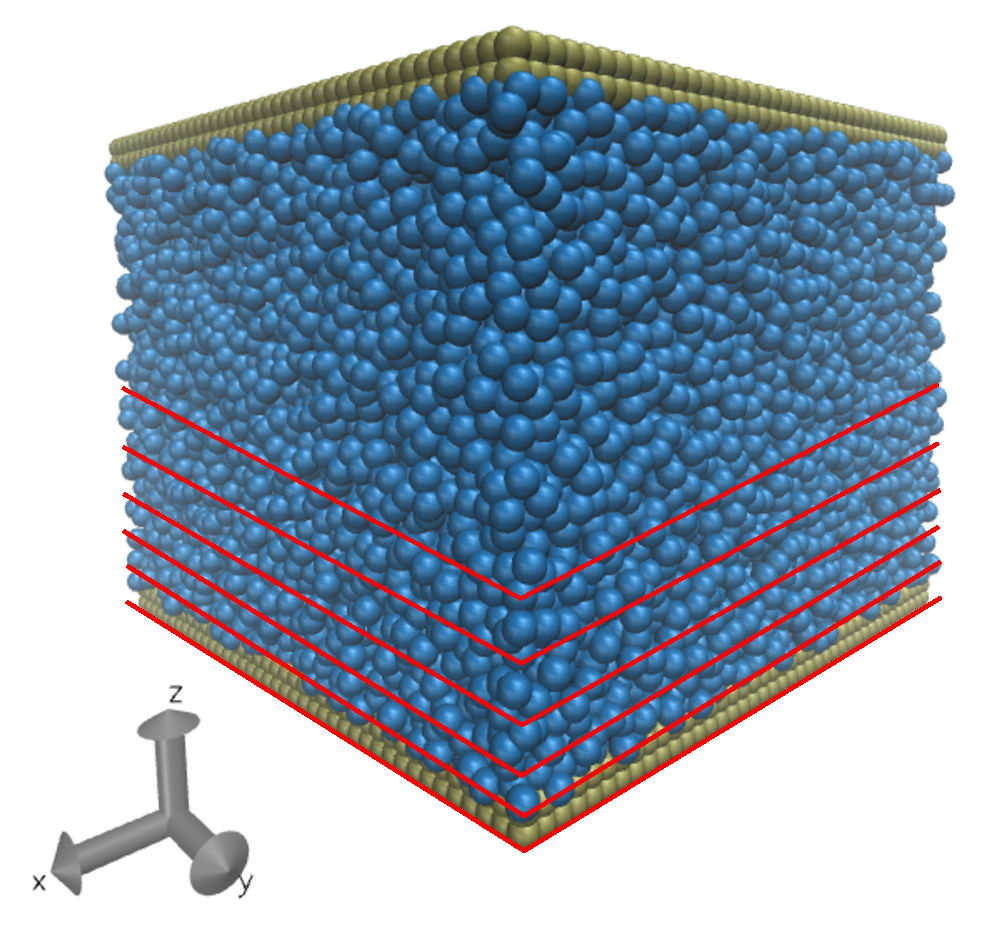
\includegraphics[scale=0.3]{system_nodes_walls}
    \caption[Walls box]{A visual representation of the MD simulation with a sketch of the binning used. In red are depicted the nodal planes used.}
    \label{fig:WallsBox}
\end{figure}

In the second publication of the series, {\it Discrete hydrodynamics II: Space and time locality for unconfined fluids}, we study through MD simulations the correlation matrix of the discrete transverse momentum density field in order to determine to what extent the Markovian approximation is valid with a non-local space description of hydrodynamics. The objetive of this publication is to understand a simpler case before moving to a system more complicated such as a fluid confined between to solid walls. 
One important learning about this publication is that we have to move to the reciprocal space (i.e. the Fourier space in the case of unconfined systems) in order to observe the time from the Markovian approximation is valid. 
The method followed in this publication will be extrapolated to the study of a confining fluids. 

In the third publication of the series, {\it Discrete hydrodynamics III: Non-Markovian behaviour near solids walls}, we perform MD simulations in order to compute the correlation matrix of the discrete transverse momentum density field of a fluid between two solid slabs. 
Because the objetive of this publication is to study the effect of the size of the bin on the Markovian behaviour near the solid walls, we discretize the system using two size of the bins. 

Finally, the objetive of the last publication of this series, {\it Discrete hydrodynamics IV: The slip boundary condition}, is to measure through MD simulations the non-local transport kernels that appear in the discrete theory presented in the first part of the series. 
We use the corrected Green-Kubo expression in order to avoid the plateu problem. 
The main result of this publication is the calculation of the slip length and the location of the hydrodynamic position of the atomic wall. We conclude that the slip lenght does not depend on the size of the channel and, therefore, it is a intrinsic surface property.  
 

%-----------------------------------------------------------------
%CHAPTER 2
%-----------------------------------------------------------------
\singlespacing
\chapter{Nanoscale hydrodynamics near solids}\label{Chap:Theory}
\markboth{Nanoscale hydrodynamics near solids}{}
\epigraph{\textit{Le temps est une invention du mouvement. Celui qui ne bouge pas ne voit pas le temps passer.}}{Métaphysique des tubes \\ AMÉLIE NOTHOMB}
\spacing{1.5}
\vspace{10pt}

\textsc{This chapter corresponds to the article \textit{Nanoscale hydrodynamics near solids} published in \textit{The Journal of Chemical Physics}. DOI:10.1063/1.5010401} 

\vspace{10pt}
In this chapter we derive DDFT for a fluid in the presence of a solid sphere. We use the projection operator technique \cite{Grabert1982} in order to obtain the hydrodynamic equations for a set of relevant variables of a system in which a fluid is in contact with a solid sphere. In order to simplify the final equations we assume the Markovian aproximation. 

\includepdf[page=-, openright=true, pagecommand={}]{00-Second-Submission26dic2017.pdf}

%-----------------------------------------------------------------
%CHAPTER 3
%-----------------------------------------------------------------
\singlespacing
\chapter{Revisiting the plateau problem in the Green-Kubo formula}\label{Chap:GKcorrected}
\markboth{Revisiting the plateau problem in the Green-Kubo formula}{}
\epigraph{\textit{Falta cita.}}{Título \\ AUTOR}
\spacing{1.5}
\vspace{10pt}

\textsc{This chapter corresponds to the article \textit{Revisiting the plateau problem in the Green-Kubo formula} published in \textit{Physical Review E}. DOI: 77777/77777} 

\vspace{10pt}
In this chapter we review the well-known plateau problem present in the Green-Kubo formulae. We use the Mori projection technique to obtain an alternative calculation of the transport coefficients expressions in which the Green-Kubo formula is corrected in a way that has no plateau problem.  

\includepdf[page=-, openright=true, pagecommand={}]{2nd-sub-GK-corrected.pdf}

%-----------------------------------------------------------------
%CHAPTER 4
%-----------------------------------------------------------------
\singlespacing
\chapter{Theory for planar flows with confinig walls}\label{Chap:Planar}
\markboth{Theory for planar flows}{}
\epigraph{\textit{Nothing got inside the head without becoming pictures.}}{The corrections \\ JONATHAN FRANZEN}
\spacing{1.5}
\vspace{10pt}

\textsc{This chapter corresponds to the article \textit{Discrete hydrodynamics I: Theory} published in \textit{Physical Review E}. DOI:77777/77777}

\vspace{10pt}
In this chapter we follow the same route established in the derivation of the hydrodynamic equations presented in the Chapter \ref{Chap:Theory}. We start from a set of discrete CG variables to derive the corresponding equations of motion.  
We also validate the final discrete equations using a Petrov-Galerkin finite element method to discretize the continuum equations obtained in Chapter \ref{Chap:Theory}.  

\includepdf[page=-, openright=true, pagecommand={}]{003-Planar-Theory-27dic2018.pdf}

%-----------------------------------------------------------------
%CHAPTER 5
%-----------------------------------------------------------------
\singlespacing
\chapter{Space and time locality for unconfined fluids}\label{Chap:PBC}
\markboth{Space and time locality for unconfined fluids}{}
\epigraph{\textit{Time is longer than any distance.}}{Absalom, Absalom! \\ WILLIAM FAULKNER}
\spacing{1.5}
\vspace{10pt}

\textsc{This chapter corresponds to the article \textit{Discrete hydrodynamics II: Space and time locality for unconfined fluids} published in \textit{Physical Review E}. DOI:77777/77777}

\vspace{10pt}
In this chapter we use the Mori theory in order to obtain the time evolution expression for the decay of the matrix of correlations of the transverse momentum of an unconfined fluid under the Markovian aproximation. We will see that if the behaviour of the fluid is Markovian, the correlations must be decay in an exponential (matrix) way after a certain time $\tau$. 

\includepdf[page=-, openright=true, pagecommand={}]{005-Mori-PBC-10oct2018.pdf}

%-----------------------------------------------------------------
%CHAPTER 6
%-----------------------------------------------------------------
\singlespacing
\chapter{Non-Markovian behaviour near solids walls}\label{Chap:Walls}
\markboth{Markovian behaviour near solids}{}
\epigraph{\textit{Descubrir es ver de otro modo lo que nadie ha percibido.}}{Blanco Nocturno \\ RICARDO PLIGIA}
\spacing{1.5}
\vspace{10pt}

\textsc{This chapter corresponds to the article \textit{Discrete hydrodynamics III: Non-Markovian behaviour near solids walls} published in \textit{Physical Review E}. DOI:77777/77777}

\vspace{10pt}
In this chapter we apply the methodology presented in the last chapter for a fluid confined between two plannar walls. 
We study the effect of the size of the bin in the Markovian behaviour of the fluid near the solid and we realize that for bins smaller than molecular dimensions the modes near the wallsare non-Markovian. 
We have to discretize the system in bigger bines to observe a Markovian behaviour of the fluid close to the solid.   

\includepdf[page=-, openright=true, pagecommand={}]{006-Mori-Correlations-Walls.pdf}

%-----------------------------------------------------------------
%CHAPTER 7
%-----------------------------------------------------------------
\singlespacing
\chapter{The slip boundary condition}
\label{Chap:Slip}
\markboth{The slip boundary condition from MD simulations}{}
\epigraph{\textit{It is remarkable how long men will believe in the bottomlessness of a pond without taking the trouble to sound it.}}{Walden \\ HENRY DAVID THOREAU}
\spacing{1.5}
\vspace{10pt}
\textsc{This chapter corresponds to the article \textit{Discrete hydrodynamics IV: The slip boundary condition} published in \textit{Physical Review E}. DOI:77777/77777}

\vspace{10pt}
In this chapter we measure the non-local transport coefficient that appear in the hydrodynamic equations derived in Chapter \ref{Chap:Planar}. Once we validate the theory we express the ``solid terms'' through a boundary condition. We infer the slip length for two system that differs in the size of the channel and conclude that it does not depende on the chanel width. 

\includepdf[page=-, openright=true, pagecommand={}]{007-BC-Simulations.pdf}


%-----------------------------------------------------------------
%CONCLUSIONS
%-----------------------------------------------------------------
\singlespacing
\chapter{Conclusions}\label{Chap:Conclusions}
\epigraph{\textit{The runner runs truly to the end.}}{Once a runner \\ JOHN L. PARKER}
\spacing{1.5}

%-----------------------------------------------------------------
%FUTURE
%-----------------------------------------------------------------
\singlespacing
\chapter{Future directions}\label{Chap:Future}
\epigraph{\textit{It's the things we forget about that tell us who we are.}}{Zero K \\ DON DELILLO}
\spacing{1.5}

\nocite{*}
%\bibliographystyle{unsrt}
\bibliographystyle{apalike}
\bibliography{../bibTex/thesis-library}

%---------
% APPENDIX
%---------
\pagestyle{noHeader}
\begin{appendices}
%\appendix
\chapter{Contributions}\label{Ap:Contributions}
The following published articles and posters are related with this dissertation.
\begin{enumerate}
  \item \cite{} Nanoscale hydrodynamics near solids.
  \item \cite{} Discrete hydrodynamics near solids for planar flows.
  \item \cite{} Revisiting the plateau problem in the Green-Kubo formula.
  \item \cite{} Space and time locality of discrete hydrodynamics.
  \item \cite{} Non-Markovian behaviour of discrete hydrodynamics near solids.
  \item \cite{} The slip boundary condition from MD simulations revisited.
  \item \cite{FISESMadrid} Nanoscale hydrodynamics in periodic and confined geometries. Poster presented at 22th Workshop on Statistical Physics (FISES18), Madrid (Spain) 2018.
  \item \cite{IWNET} Nanoscale hydrodynamics in periodic boundary conditions. Poster presented at 8th International Workshop on Nonequilibrium Thermodynamics, Sint-Michielsgestel (The Netherlands) 2018.
  \item \cite{Ulam} Nanoscale heat transport in fluids near solids. Poster presented at Ulam Computer Simulation Workshop, Lviv (Ukraine) 2017.
  \item \cite{FISESSevilla} Thermal hydrodynamics transport between fluids and solids. Poster presented at 21th Workshop on Statistical Physics (FISES17), Seville (Spain) 2017.
  \end{enumerate}

  Furthemore, I presented part of this work in two seminars at the National University of Distance Education. 
  \begin{enumerate}
  \item Nanoscale hydrodynamics nears solids. National University of Distance Education, Madrid (Spain) 2017.
              \item Simulación de procesos térmicos en la dinámica de nanofluidos. National University of Distance Education, Madrid (Spain) 2016.
  \end{enumerate}

\chapter{List of Acronyms}\label{Ap:Acronyms}
\begin{tabular}{l l}
    CM   & Classical Mechanics \\
    DFT  & Density Functional Theory \\
    DDFT & Dynamic Density Functional Theory \\
    GLE  & Generalized Langevin Equation \\
    LADM & Local Average Density Model \\
    LJ   & Lennard-Jones \\
    LFSA & Linear For Spiky Approximation \\
    MD   & Molecular Dynamics \\
    NEMD & Non-Equilibrium Molecular Dynamics\\
    NESM & Non-Eauilibrium Statistical Mechanics \\
    QM   & Quantum Mechanics \\
    SM   & Statistical Mechanics \\
    ToCG & Theory of Coarse-Graining \\
\end{tabular}


\chapter{Physical parameters and variables}
\begin{tabular}{l l}
    $m$ & mass particles \\
    $L_x, L_y, L_Z$ & dimensions of the simulations box \\
    $M'$ & mass solid sphere \\
    $M$ & mass solid walls \\
    $N$ & Number of liquid particles \\
    $N'$ & Number of solid particles \\
    $N_{\rm bins}$ & Number of bins \\
    $k_B$ & Boltzmann's constant \\
    $T$ & Temperature \\
    $\beta$ & $(k_BT)^{-1}$ \\
    $\Delta z$ & distance between two nodal planes \\
    $\delta_{\mu\nu}$ & Kronecker delta \\
    ${\cal F}[]$ & Free energy functional \\
    $F()$ & Free energy function \\
\end{tabular}
\end{appendices}

\end{document}
